\chapter{Linear Bayesian vs. Regularisation -- Ozone}
\label{ch:LinVsReg}
\thispagestyle{empty}

In this Chapter, we guide the reader through the process of setting up a hierarchical Bayesian framework, establishing a choice of prior distributions, and using a DAG to visualise conditional dependencies between hyper-parameters and parameters.
Applying the MTC scheme the marginal and then full conditional posterior distributions are explicitly formulated.
Here this inverse problem is treated as a linear inverse problem by neglecting the absorption term in RTE (see Eq.~\ref{eq:RTE}).
A Metropolis within Gibbs sampler and a TT approximation to characterise the marginal posterior are utilised.
Then we calculate the mean and the covariance matrix of the posterior distribution for ozone and compare it to a regularisation approach.


\section{Hierarchical Bayesian Framework}
\label{sec:BayModelO3}
\begin{figure}[htb!]
	\centering
	\begin{tikzpicture}
		%box/.style = {draw, thick, minimum width=2.5cm, minimum height=1cm},
		every edge/.style = {draw, -latex, thick} % <---
		\node[roundnode2] at (-4,6.5) (Q)     {$\bm{Q}$};
		\node[roundnode2] at (-2.5,5) (x)     {$\bm{x}$};
		\node[align=center] at (-1,4) (A)    {$\bm{A}$};
		\node[roundnode2] at (-1,2.5) (u)    {$\Omega$};
		\node[rectnode] at (-1,1) (y)    {$\bm{y}$};
		\node[roundnode2] at (-2.5,2.5) (e)    {$\bm{\eta}$};
		\node[roundnode2] at (-6.5,6.5) (S)    {$\bm{\Sigma}$};
		\node[roundnode2] at (-8,8) (s)    {$\gamma$};
		\node[roundnode2] at (-5.5,8) (d)    {$\delta$};
		
		\node[roundnode2] at (-8,10) (shyp)    {$\bm{\theta}_{\gamma}$};
		\node[roundnode2] at (-5.5,10) (dhyp)    {$\bm{\theta}_{\delta}$};
		%Lines
		\draw[->, very thick] (S) -- (e);
		\draw[->, mydotted, very thick] (s) -- (S);
		\draw[->, mydotted, very thick] (e) -- (y);
		\draw[->, very thick] (u.south) -- (y);
		\draw[->, mydotted, very thick] (A) -- (u);
		\draw[->, mydotted,  very thick] (x) -- (A.west);
		\draw[->, very thick] (shyp) -- (s);
		\draw[->, very thick] (dhyp) -- (d);
		
		
		\draw[->, mydotted, very thick] (d) -- (Q); 
		
		\draw[->, very thick] (Q) -- (x); 
		%\node[align=center] at (0,4) (f3) {$= \bm{A}$};
		%\node[align=center] at (0.25,3.95) (f3) {$\approx \bm{M A}_L$};
		\node[align =center] at (-2,8) (T1) {marginal posterior \\ over hyper-parameters \\ $\pi(\delta,\gamma  | \bm{y})$};
		\node[align =center] at (0,5) (T2) {full conditional \\ posterior \\ $\pi( \bm{x} | \delta,\gamma, \bm{y})$ };
		
		%\node[align =center] at (-2.5,10) (T3) {hyper-prior distributions \\ $\pi( \delta, \gamma)$ };
		
		\node[fit=(s)(d),draw,dotted,black, rounded corners] {};
		\draw[->,dotted] (y) edge[bend right=85] (T1);  
		\draw[->,dotted] (T1) -- (T2); 
		
	\end{tikzpicture} 
	\caption[Directed acyclic graph for ozone retrieval and MTC scheme.]{DAG for visualisation of hierarchical modelling and measuring process of ozone, including the MTC scheme. The hyper-parameter $\gamma$ deterministically (dotted line) sets the noise covariance $\bm{\Sigma} = \gamma^{-1}\bm{I}$ and hence the random (solid line) noise vector $\bm{\eta} \sim \mathcal{N}(0, \gamma^{-1}\bm{I})$.
		The hyper-parameter $\delta$ determines (dotted line) the prior precision matrix $\bm{Q} = \delta \bm{L}$ for the normally distributed (solid line) prior $\bm{x}| \delta \sim \mathcal{N}(0, \delta \bm{L})$, where $\bm{L}$ is a graph Laplacian, see Eq.~\ref{eq:GLapl}.
		The hyper-prior distributions (solid line) $\pi(\delta, \gamma)$ are defined by $\bm{\theta}_{\gamma}$ and $\bm{\theta}_{\delta}$.
		Through a linear forward model $\bm{A}$, we generate a space of all measurable noise-free data $\bm{A}\bm{x}$ from which we randomly observe a data set $\bm{y}$ including some added noise $\bm{\eta}$.
		Within the MTC scheme, we evaluate the marginal posterior over the hyper-parameters $\pi(\gamma, \delta | \bm{y})$ first and then the full conditional posterior $\pi(\bm{x}|\delta,\gamma,\bm{y})$. This breaks the correlation structure of $\bm{x}$ and $\delta$ and $\gamma$, and allows us to evaluate the marginal posterior independent of $\bm{x}$.}
	\label{fig:DAGO3}
\end{figure}
In this section, we set up the hierarchically-ordered linear-Gaussian Bayesian framework to determine the ozone posterior distribution, conditioned on ground truth temperature and pressure.
For now the forward model matrix is defined as $\bm{A} \coloneqq \bm{A}_L$ and the distributions of that Bayesian model are:
\begin{subequations}
		\label{eq:O3BayMode}
	\begin{align}
		\bm{y} |  \bm{x},\gamma,\delta  &\sim \mathcal{N}(\bm{A} \, \bm{x}, \gamma^{-1} \bm{I}) \label{eq:likelihoodAppl} \\
		\bm{x}| \delta  &\sim \mathcal{N}(\bm{0}, (\delta \bm{L})^{-1} ) \label{eq:priorXAppl} \\
		\delta  &\sim \Gamma(\alpha_{\delta}, \beta_{\delta})\label{eq:priorDelAppl} \\
		\gamma  &\sim \Gamma(\alpha_{\gamma}, \beta_{\gamma})\label{eq:priorGamAppl} \, .
	\end{align} 
\end{subequations}
Assuming Gaussian noise $\bm{\eta} \sim \mathcal{N}(0, \gamma^{-1} \bm{I})$, the likelihood function is a normal distribution with mean $\bm{A} \bm{x}$ and covariance matrix $\gamma^{-1} \bm{I}$.
We define the normal prior-distribution $\pi(\bm{x}|\delta)$ with zero mean and precision matrix $\delta \bm{L}$, where $\delta$ is a smoothness hyper-parameter and $\bm{L}$ is a discrete approximation to the second derivate operator (see Eq.~\ref{eq:GLapl}).
Here the hyper-prior distributions $\pi(\delta)$ and $\pi(\gamma)$ are gamma distributions with shape $\alpha$ and rate $\beta$.

We can visualise this hierarchical structure and the conditional dependencies between hyper-parameters and parameters through a DAG, as in Fig.~\ref{fig:DAGO3}.
The hyper-parameter $\gamma$ sets the noise covariance deterministically (dotted line), but is itself statistically (solid line) defined by the hyper-prior distribution $\pi(\gamma)$.
This is a gamma distribution, where $\bm{\theta}_{\gamma}$ determines the shape and rate of $\pi(\gamma)$.
Similarly $\bm{\theta}_{\delta}$ defines $\pi(\delta)$, where $\delta$ accounts for smoothness of the ozone profile and sets the prior precision $\bm{Q}(\delta)$.
Then $\bm{A}\bm{x}$ determines the space of all measurable noise-free data sets $\Omega$ through the linear forward model, from which we observe a data set $\bm{y}$ including some noise $\bm{\eta}$.
Given that data, we ``reverse the arrows'' to determine the posterior distribution $\pi(\bm{x}, \bm{\theta}|\bm{y})$ over the parameter $\bm{x}$ and the hyper-parameters $\bm{\theta}$.
%Since noise is a random process with a defined distribution, the posterior distribution $\pi(\bm{x}|\bm{y})$ is well defined.
Usually, due to underlying correlation structures, evaluating this posterior poses a signifiant challenge.
The MTC scheme breaks this correlation and provides the marginal posterior $\pi(\delta, \gamma | \bm{y})$ first and then the full conditional posterior $\pi(\bm{x}|\delta, \gamma,\bm{y})$.
%Since the forward model described in Ch. \ref{ch:formodel} is weakly non-linear we will set up a linear Bayesian hierarchical framework first based on the linear forward model $\bm{A}_L$ and then later the approximated version $\bm{A}_{NL}\bm{M} \bm{A}_L$.
%Furthermore, the noise is normally distributed, so we establish a linear-Gaussian Bayesian hierarchical framework, aiming to recover an ozone profile and a pressure over temperature profile.
%In doing so, we first draw a directed acyclic graph (DAG) to visualise the measurement and modelling process and determine hyper-parameters and correlations between parameters.
%Then we define prior distributions over all parameters as well as a likelihood function so that we can formulate the posterior distribution.

%In this section, we choose the prior distributions and describe the approach to evaluate the posterior distribution for ozone $\pi(\delta, \gamma, \bm{x}|\bm{y})$, including the noise hyper-parameter $\gamma$.
% we define a linear-Gaussian Bayesian hierarchical model, see Sec. \ref{subsec:LinBay},
%\begin{subequations}
%	\begin{align}
	%		\bm{y} |  \bm{x}, \gamma &\sim \mathcal{N}(\bm{A} \bm{x}, \gamma^{-1} \bm{I}) \label{eq:likelihood} \\
	%		\bm{x} |  \delta &\sim \mathcal{N}(\bm{0}, (\delta \bm{L})^{-1}) \label{eq:xPrior} \\
	%		\delta, \gamma &\sim \pi(\delta, \gamma) \label{eq:gammaPrior},
	%	\end{align}
%	\label{eq:O3BayMode}
%\end{subequations}
%with a normally distributed likelihood $\pi(\bm{y} |  \bm{x}, \gamma)$ including the forward model matrix $\bm{A}$ and prior distributions $\pi(\bm{x} |  \delta)$ and $\pi(\delta, \gamma)$, the noise covariance matrix $\gamma^{-1} \bm{I}$, the prior precision matrix $\delta \bm{L}$ and the prior mean set to zero, as in ~\cite{fox2016fast}.
%The chosen Bayesian model is very similar to the regularisation approach, since we like to show that we receive much more meaningful results compared to a single regularisation solution.

\subsection{Prior Modelling}
\label{subsec:PriorModelO3}
To complete the Bayesian framework, we have to define prior distributions over the hyper-parameters and parameters.
Ideally, we define the prior distributions as uninformative as possible, and include functional dependencies and physical properties.

By choosing a normally distributed prior $\pi(\bm{x}|\delta)$ with zero mean and no other restrictions, it is clear that our model does not take into account that ozone values cannot be negative.
As already mentioned, we set the precision matrix of that prior distribution to
\begin{align}
	\delta \bm{L} =
	\delta
	\begin{bmatrix}
		2 & -1 & & &  \\
		-1 & 2 & -1 & &   \\
		& \ddots & \ddots & \ddots &\\ 
		& & -1 & 2 & -1  \\
		& & & -1 & 2 
	\end{bmatrix} 
	\label{eq:GLapl} 
\end{align}
which is discrete approximation to the second derivate operator with Dirichlet boundary condition and defines a 1-dimensional Graph Laplacian as in~\cite{wang2015graphs, fox2016fast}.
This matrix will also act as the regulariser later in Sec.~\ref{sec:SolByReg}.
We reduce the dimension of $\bm{x}$ from $45$ to $34$ by discarding every second ozone VMR over a height of $\approx47$km.
Doing that, while not changing $\bm{L}$, we effectively induce a larger correlation between points at higher altitude.
We plot the corresponding prior ozone profiles according to $\bm{x}\sim \mathcal{N}(0, (\delta \bm{L})^{-1})$ in Fig.~\ref{fig:O3Prior}.

For $\delta$ and $\gamma$ we pick relatively uninformative gamma distributions so that $\gamma \sim \mathcal{T}(\bm{\theta_{\gamma}}) \propto \gamma^{\alpha_\gamma -1 } \exp{( -\beta_\gamma \gamma) } $ and $\delta \sim \mathcal{T}(\bm{\theta_{\delta}})$, where $\bm{\theta_{\gamma}} = \{  \alpha_\gamma, \beta_\gamma\}  = \{ \alpha_\delta ,\beta_\delta\} = \bm{\theta_{\delta}} = (1,10^{-35})$ (see Fig.~\ref{fig:MargPostHistTT}) similar to \cite{fox2016fast}.
Those gamma distributions have another advantage when using the Metropolis within Gibbs algorithm, as in Sec.~\ref{subsec:MWG} to sample from the marginal posterior distribution $\pi(\delta, \gamma | \bm{y})$, where then $\pi(\gamma | \lambda, \bm{y}) \sim \mathcal{T}(\cdot)$ is a gamma distribution with $\lambda = \delta / \gamma $, and easy to sample from.

\section{Posterior Distribution}
\label{sec:FirstO3Post}
As explained in Sec.~\ref{subsec:TheoMTC},we factorise the posterior
\begin{align}
	\pi( \bm{x}, \delta, \gamma| \bm{y}) \propto \pi(\bm{y}| \bm{x},\delta,\gamma) \pi( \bm{x},  \delta,\gamma)
\end{align}
into 
\begin{align}
	\pi( \bm{x},  \delta,\gamma| \bm{y}) =\pi( \bm{x}| \delta,\gamma, \bm{y})\pi( \delta,\gamma | \bm{y})
\end{align}
the marginal posterior $\pi(\delta ,\gamma| \bm{y})$ and full conditional posterior $\pi( \bm{x}| \delta,\gamma, \bm{y})$ (see Eq.~\ref{eq:MTC}).
%Fox and Norton call this method the marginal and then conditional method (MTC) \cite{fox2016fast}, where we break the correlation structure between $\bm{x}$ and $\gamma, \delta$ as illustrated in Fig. \ref{fig:RueHeld} by marginalising over $\bm{x}$.
As discussed in Sec.~\ref{subsec:LinBay}, for the linear-Gaussian case, $\bm{x}$ cancels in the marginal posterior over the hyper-parameters.
Following the MTC scheme, we characterise the marginal posterior first and then the full conditional posterior.

\subsection{Marginal Posterior}
\label{subsec:FirstMargPost}
Consequently, for the hierarchical model specified in Eq.~\ref{eq:O3BayMode}, the marginal posterior distribution over the hyper-parameters is given by
\begin{align}
	\pi( \lambda,\gamma  | \bm{y}) \propto &  \lambda^{n/2 + \alpha_{\delta}-1} \gamma^{m/2 + \alpha_{\delta} + \alpha_{\gamma}-1}   \exp{ \Bigl\{ - \frac{1}{2} g ( \lambda) - \frac{\gamma}{2} f ( \lambda) - \beta_{\delta} \lambda  \gamma - \beta_{\gamma} \gamma \Bigr\}},
	\label{eq:MargPostAppl}
\end{align}
with the introduced regularisation parameter $\lambda = \delta / \gamma$, and
\begin{subequations}
	\begin{align}
		&f ( \lambda) = \bm{y}^T \bm{y} - (\bm{A}^T \bm{y})^T (\bm{A}^T  \bm{A} + \lambda \bm{L})^{-1} (\bm{A}^T \bm{y})  \label{eq:fAppl} \, ,  \\
		&\text{and } g(\lambda) = \log \det (\bm{A}^T  \bm{A} + \lambda \bm{L}) \label{eq:gAppl} \, .
	\end{align}
\end{subequations}
Note that when changing variables from $\delta = \lambda \gamma$ to $\lambda$ the hyper-prior distribution changes to $\pi(\lambda) \propto \lambda^{\alpha_{\delta}-1} \gamma^{\alpha_{\delta}} \exp{(- \beta_{\delta} \lambda  \gamma)} $, due to $\text{d}\delta / \text{d} \lambda = \gamma$.
\begin{figure}[th!]
	\centering
	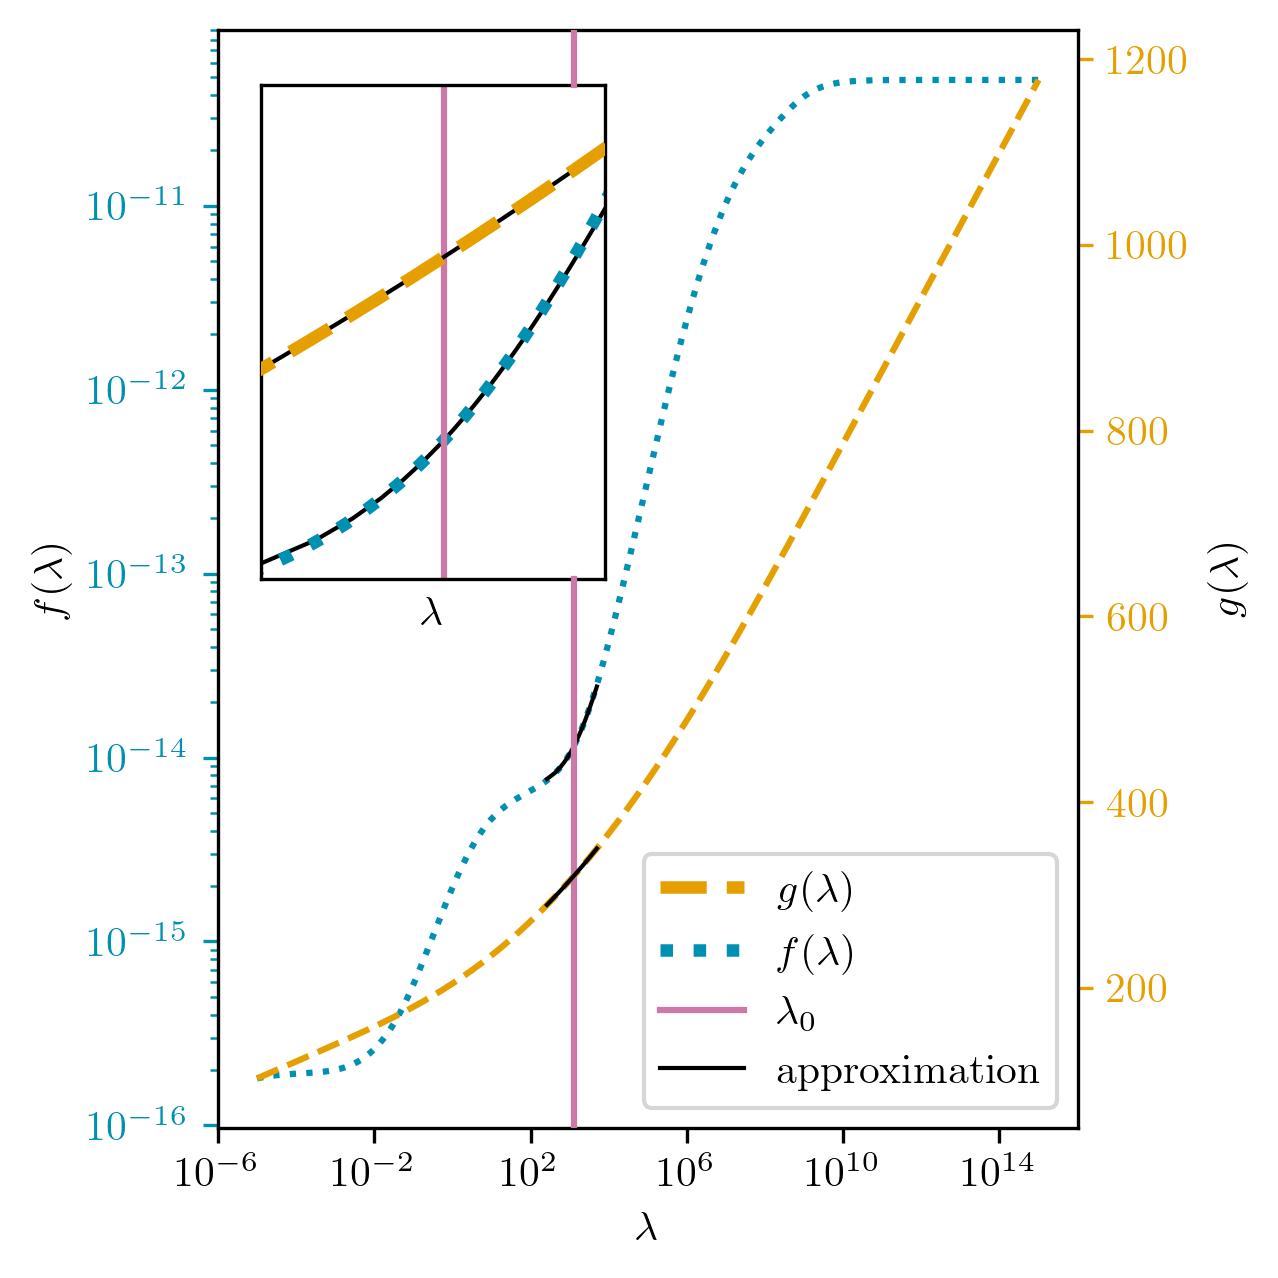
\includegraphics{f_and_g_phd.png}
	\caption[Functions $f(\lambda)$ and $g(\lambda)$ of 2D marginal posterior.]{Functions $f(\lambda)$ and $g(\lambda)$ from the marginal posterior in Eq.~\ref{eq:MargPostAppl} for a wide range of $\lambda = \delta / \gamma$. We plot the approximations (see Eq.~\ref{eq:fAprox} and Eq.~\ref{eq:gAprox}) in black around the mode of the marginal posterior (vertical line) for the sampling range of $\lambda$ within the MWG algorithm.}
	\label{fig:fandg}
\end{figure}
For each evaluation of the marginal posterior most of the computational effort lies in the calculation of $f(\lambda)$ and $g(\lambda)$.
Obtaining the Cholesky decomposition $\bm{A}^T  \bm{A} + \lambda \bm{L} = \bm{C}_{\lambda} \bm{C}_{\lambda}^T$ via \texttt{numpy.linalg.cholesky} immediately gives $g(\lambda) = 2 \sum \log \text{diag}(\bm{C}_{\lambda}) $.
Additionally to the Cholesky decomposition of $\bm{A}^T  \bm{A} + \lambda \bm{L}$, the Python function \texttt{scipy.linalg.cho\_solve} is used to solve for $(\bm{A}^T  \bm{A} + \lambda \bm{L})^{-1} (\bm{A}^T \bm{y})$ to calculate $f(\lambda)$.
If that is not too expensive one may consider a 
In  Fig.~\ref{fig:fandg} we see that $f(\lambda)$ and $g(\lambda)$ are well behaved within the region of interest.
Because of this, we approximate $f(\lambda) \approx \tilde{f}(\lambda)$ with a Taylor series and $\tilde{g}(\lambda) \approx g(\lambda)$ with a linear approximation in $\lambda$ log-space around the mode $\lambda_0$ of $\pi(\lambda, \gamma | \bm{y})$.
The Taylor series coefficient of $f(\lambda)$ is given by
\begin{align}
	f^{(r)}& (\lambda_0)= (-1)^{r+1} (\bm{A}^T \bm{y})^T (\bm{B}_0^{-1} \bm{L})^r \bm{B}_0^{-1} \bm{A}_L^T \bm{y} \label{eq:ftay} 
\end{align} 
with $\bm{B}_0 = \bm{A}^T  \bm{A} + \lambda_0 \bm{L}$.
Note that usually a Taylor series includes a factor $(r!)^{-1}$~\cite{fox2016fast}, which in this case cancels in $f^{(r)}(\lambda_0)$ so that $f(\lambda)$ is approximated as 
\begin{align}
		\tilde{f} ( \lambda) = \sum^{\infty}_{r=0} 	f^{(r)}(\lambda_0) (\lambda-\lambda_0)^r  \label{eq:fAprox} \, . 
\end{align}
By exploratory analysis we find that the approximation
\begin{align}
 \tilde{g}(\lambda)=  g(\lambda_{0}) + (\log{\lambda} - \log{\lambda_{0}})  \frac{ g(1.25\lambda_{0}) - g(0.75\lambda_{0}) }{\log{1.25\lambda_{0}} - \log{0.75\lambda_{0}} }  \label{eq:gAprox} \, 
\end{align}
is sufficient.
Note that $g(\lambda)$ can be approximated with a Taylor series as well (see~\cite{fox2016fast}).
We plot the function $f(\lambda)$ and $g(\lambda)$ and their approximations in Fig.~\ref{fig:fandg} and elaborate on the approximation errors in the section below.

\subsubsection{Error due to approximation of f and g}
To assess the approximation error, we lay a 100-point grid over the sampling region in each dimension and compare the approximations of $f(\lambda)$, $g(\lambda)$ and $\pi(\lambda, \gamma | \bm{y})$ with their true function values.

Compared to a 2nd, 3-rd or 4-th order Taylor approximation, the 1-st order Taylor approximation of $f(\lambda)$ gives the smallest relative RMS error of $\approx 9 \%$ for $\lambda = [ 10^{-5}, 8 \times 10^{-4}]$ (TT grid) and a maximum absolute error of $\approx 3 \times 10^{-16}$.
Additionally, the linear approximation of $g(\lambda)$ has a relative RMS of $\approx 3\%$ and a maximum absolute error of $\approx 5$.

These errors then propagate into the marginal posterior $\pi(\lambda , \gamma| \bm{y})$ so that the relative RMS error is $\approx 6 \%$ over the whole grid.
When sampling, we evaluate the acceptance ratio in the log-space, so we report a relative RMS error of $ \approx0.1\%$ for $\log{\pi(\lambda| \gamma, \bm{y})}$.
We consider this good enough.




\subsubsection{Sample from marginal posterior -- Metropolis within Gibbs}
\label{subsec:MWG}
Using these approximations, a Metropolis within Gibbs (MWG) sampler summarised in Alg. Box \ref{alg:MwG} is employed to characterise $\pi(\lambda,\gamma|\bm{y})$ as in~\cite{fox2016fast}.
More specifically, we implement a Metropolis random walk on
\begin{align}
	\label{eq:margApplCondGam}
	\pi(\lambda | \gamma, \bm{y}) &\propto \lambda^{n/2 +\alpha_{\delta}-1} \exp{\Bigl\{ - \frac{1}{2} g ( \lambda) - \frac{\gamma}{2} f ( \lambda) - \beta_\delta \gamma \lambda \Bigr\}}
\end{align} 
and do a Gibbs step on
\begin{align}
	\gamma |  \lambda, \bm{y} &\sim \Gamma \bigg( \frac{m}{2} + \alpha_\delta + \alpha_\gamma, \frac{1}{2} f (\lambda + \beta_\gamma + \beta_\delta \lambda \bigg)\label{eq:GibbsStep} \ .
\end{align} 
Ergodicity for this approach is proven in~\cite{roberts2006harris}.

\begin{algorithm}[!ht]
	\caption{Metropolis within Gibbs}
	\begin{algorithmic}[1]
		\STATE Initialise \( ( \lambda_1^{(0)} , \gamma_2^{(0)}  )= ( \lambda_{0} , \gamma_{0}  )  \)
		\FOR{ \( k = 0, \dots, N-1 \)}
		\STATE Propose \( \lambda^{\prime} \sim q(\cdot   | \lambda^{(k)}) = q(\lambda^{(k)} |\cdot  ) \)
		\STATE Compute
		\[ \alpha( \lambda^{\prime} | \lambda^{(k)}) = \min \left\{ 1, \frac{\pi(\lambda^{\prime}  | \gamma^{(k)}, \bm{y}) \cancel{q(\lambda^{(k)} | \lambda^{\prime} ) } }{\pi(\lambda^{(k)} | \gamma^{(k)}, \bm{y}) \cancel{q(\lambda^{\prime} | \lambda^{(k)})} } \right\} \]
		\STATE Draw $u \sim \mathcal{U}(0,1)$
		\IF{$\alpha \geq u$ }
		\STATE Accept and set \( \lambda^{(k+1)} = \lambda^{\prime} \)
		\ELSE  
		\STATE Reject and keep \(\lambda^{(k+1)} = \lambda^{(k)} \)
		\ENDIF
		\STATE Draw \(\gamma^{(k+1)} \sim  \pi( \cdot | \lambda^{(k+1)} , \bm{y} )\) 
		\ENDFOR
		\STATE Output: $ (\lambda,\gamma)^{(0)}, \dots,  (\lambda,\gamma)^{(k)} , \dots,   (\lambda,\gamma)^{(N)} \sim \pi(\bm{\theta}| \bm{y}) $
	\end{algorithmic}
	\label{alg:MwG}
\end{algorithm}


The MWG algorithm starts at the initial guess $( \lambda^{(0)} , \gamma^{(0)}  )$ at $k=0$. We then propose a new sample $\lambda^{\prime} \sim q(\cdot |  \lambda^{(k)})$, conditioned on the previous state, using a symmetric proposal distribution $q(\lambda^{\prime} |  \lambda^{(k)}) = q(\lambda^{(k)} |  \lambda^{\prime})$, which is a Metropolis step and a special case of the Metropolis-Hastings algorithm~\cite{roberts2006harris}.
We accept and set $\lambda^{(k+1)} = \lambda^{\prime}$ with the acceptance probability
\begin{align}
\alpha( \lambda^{\prime} | \lambda^{(k)}) = \min \left\{ 1, \frac{\pi(\lambda^{\prime}  | \gamma^{(k)}, \bm{y}) \cancel{q(\lambda^{(k)} | \lambda^{\prime} ) } }{\pi(\lambda^{(k)} | \gamma^{(k)}, \bm{y}) \cancel{q(\lambda^{\prime} | \lambda^{(k)})} } \right\} \, ,
\end{align}
otherwise reject and keep $\lambda^{(k+1)} = \lambda^{(k)}$.
In practice, we calculate the acceptance ratio in log-space, so that
\begin{align} 
	\log \left\{ \frac{\pi(\lambda^{\prime} | \gamma^{(k)}, \bm{y})  }{\pi(\lambda^{(k)}| \gamma^{(k)}, \bm{y})}  \right\} 
	= \log  \{\pi(\lambda^{\prime} | \gamma^{(k)}, \bm{y} ) \}  -\log  \{ \pi(\lambda^{(k)}| \gamma^{(k)}, \bm{y}) \} \\
	= \frac{n}{2} (\log\{\lambda^{\prime}\} - \log\{\lambda^{(k)}\} ) + \frac{1}{2} \Delta g + \frac{\gamma^{(k)}}{2} \Delta f  + \beta_\delta \gamma^{(k)} \Delta \lambda  \, ,
\end{align}
where $\Delta \lambda = \lambda^{\prime} - \lambda^{(k)} $ and  $\Delta f \approx  \tilde{f} (\lambda^\prime) - \tilde{f}(\lambda^{(k)}) =   f^{(1)}(\lambda_0) \Delta \lambda^\prime- \Delta \lambda^{(k)} $, with  $\Delta \lambda^{\prime} = \lambda^\prime - \lambda_0 $ and $\Delta \lambda^{(k)} =  \lambda^{(k)} - \lambda_0$.
Similarly we approximate $\Delta g \approx \tilde{g}(\lambda^{\prime}) -\tilde{g}(\lambda^{(k)})$.

Next, we perform a Gibbs step on $\pi(	\gamma^{(k+1)} |  \lambda^{(k+1)}, \bm{y}) $ conditioned on the prevously drawn $ \lambda^{(k+1)}$.
Gibbs sampling is again a special case of the Metropolis-Hastings algorithm with  acceptance probability equal to one.
Repeating this N time give us marginal posterior samples $(\lambda, \gamma)^{(1)}, \dots, (\lambda, \gamma)^{(N)} \sim  \pi(\lambda, \gamma| \bm{y})$.
For we discard the first $N_{\text{burn-in}}$ samples.


To run the MWG sampler we firstly approximate $f(\lambda)$ and $g(\lambda)$ around the mode $( \lambda_{0}, \gamma_0 )$ of $\pi(\lambda,\gamma| \bm{y})$ as previously described. 
The mode is provided by the \texttt{scipy.optimize.fmin} function, with a limit of 25 function evaluations.
Initialised at the mode $(\lambda^{(0)} , \gamma^{(0)}  ) = ( \lambda_{0} , \gamma_{0}  )$ the MWG sampler takes $N = 10100$ , which includes burn in period of $N_{\text{burn-in}} = 100$ steps.
The standard deviation of the normal proposal distribution $\lambda^{\prime} \sim \mathcal{N}(\lambda^{(k)} , \sigma^2_{\lambda})$ is empirically set to $\sigma_{\lambda} = 0.8 \lambda_0$, so that the acceptance rate is $\approx 0.5$ as suggested in~\cite{robertsLecNot}.
This takes  $\approx 0.5$s and we plot in Fig.~\ref{fig:ScatterPlotTT} as well as the trace of the MWG to show ergodicity.
The IACTs is given by twice the value of the Python implementation of~\cite{wolff2004monte} provided by~\cite{drikHesse}, so that $\tau_{\text{int}, \gamma} \approx 4.4 \pm 0.2$ and $\tau_{\text{int}, \lambda} = 10.4 \pm 1.0 $ (see Fig.~\ref{fig:IATCLamLin} and Fig.~\ref{fig:IATCGamLin}).
\begin{figure}[h!]
	\centering
	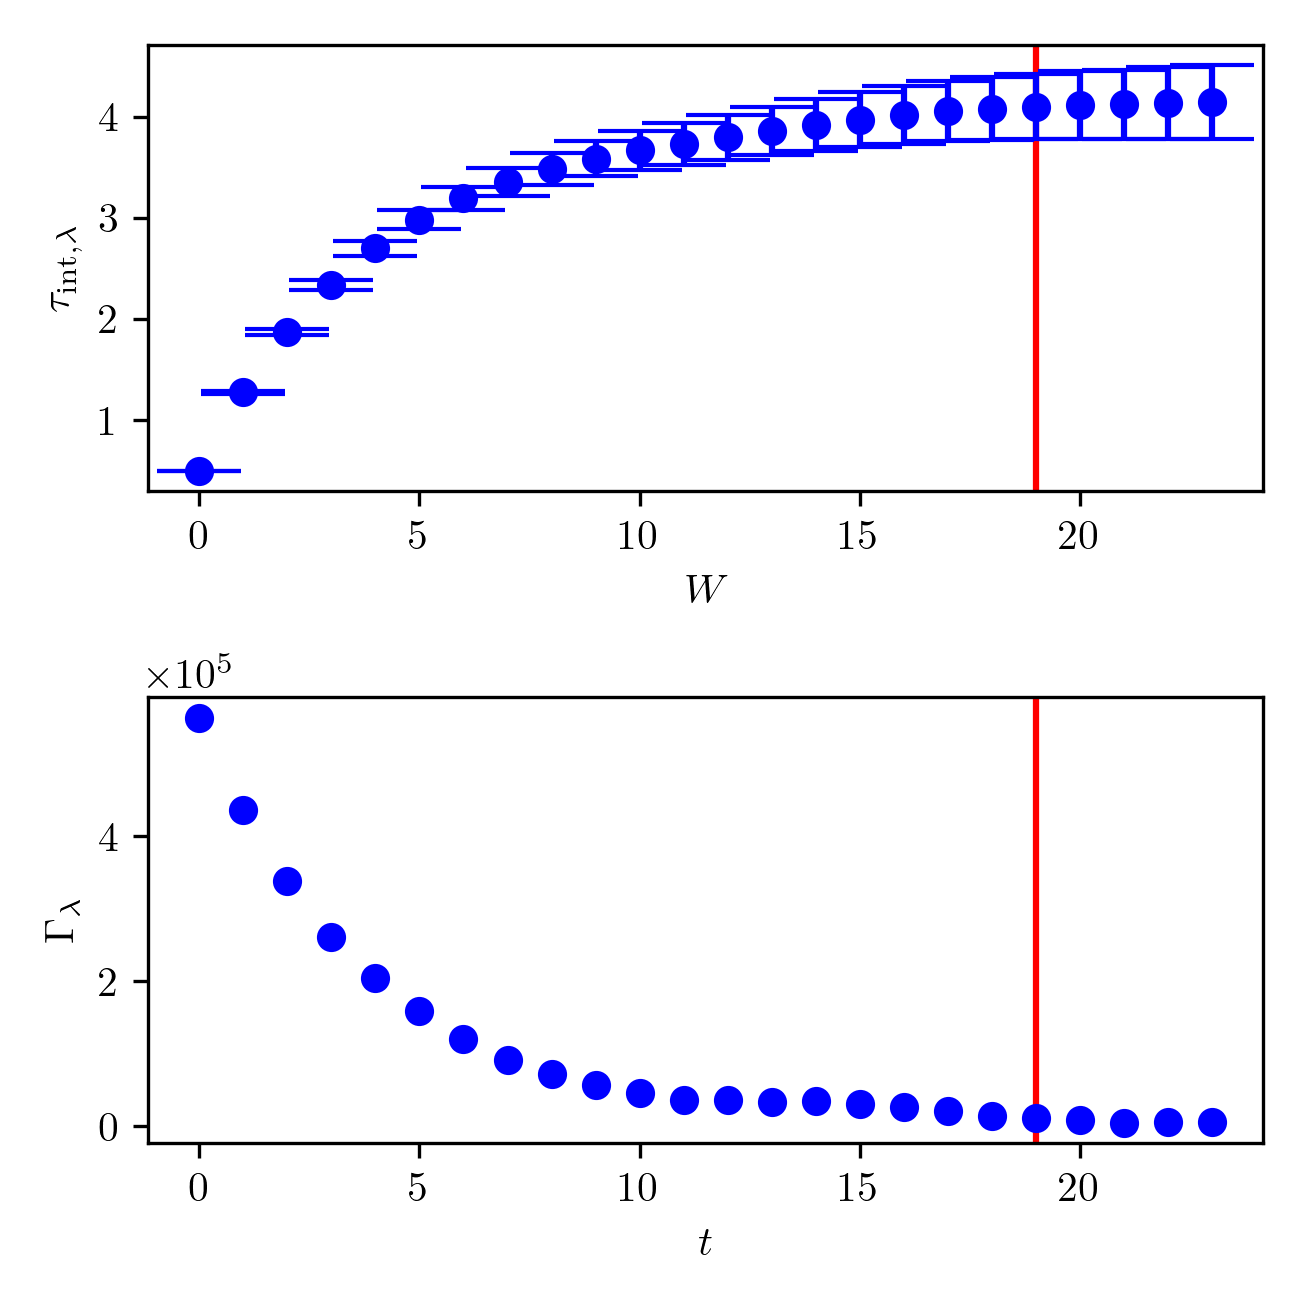
\includegraphics{UwerrTauIntFirstO3lam.png}
	\caption[IACT of $\lambda \sim \pi( \cdot| \bm{y})$, for linear model.]{Provided by \cite{drikHesse}, the IACT $\tau_{\text{int},\lambda}$ at summation windows W as well as the estimated autocorrelation function $\Gamma_{\lambda}$ at lag $t$ of the samples $\lambda \sim \pi( \cdot| \bm{y})$.}
	\label{fig:IATCLamLin}
\end{figure}


\subsubsection{TT approximation of marginal posterior}
Alternatively, we can utilise a TT approximation of the square root of the marginal posterior over a predefined grid and calculate the marginals $\pi(\gamma|\bm{y})$ and $\pi(\lambda|\bm{y})$ (see Sec. \ref{subsec:TTMarg}).

We predefine the univariate grid with $n = 20$ grid points (see Fig. \ref{fig:MeanVarError}) over $\gamma = [ 0.8 \times 10^{15},1.2 \times 10^{16}]$ and $\lambda = [ 10^{-5}, 8 \times 10^{-4}]$.
The ``normalisation constant'' is set to $c=-150$ so that the values of $\sqrt{\pi( \lambda,\gamma| \bm{y})} = \exp \{ 0.5 \log  \pi(\lambda,\gamma | \bm{y}) + c \} $ are within computer precision.
 %-320/2
Then we initialise the~\texttt{tt.cross.rectcross.rect\_cross.cross} function based on the TT cross algorithm in \cite{OSELEDETS2010TTCross,Dolgov2018TTCross} from the Python package \texttt{ttpy}~\cite{Oseledets2018ttpy} with a random tensor.
The number of ranks $r = 4$ is constant and we do one sweep with $2n_{\text{sweeps}}2nr =400$ function evaluations and obtain a TT approximation of $\pi( \lambda,\gamma| \bm{y})$ in about $0.02$s.
Ironically, this the same number of functions evaluations to approximate a $20 \times 20$ point grid.
The TT format is especially advantageous for larger grid sizes and higher dimensional parameter spaces.
To compute the marginals $\pi(\lambda| \bm{y})$ and $\pi(\gamma| \bm{y})$ we set the TT error $\xi = 1 / \uplambda (\mathcal{X})$ and $\uplambda(x) = 1$, so that for Cartesian basis $\bm{M}_k = \text{diag}(\uplambda_k(\mathcal{X}_k))$ (see Eq.~\ref{eq:MassMat}).
We calculate the coefficient tensor $\bm{B}$ and $\bm{R}_{\text{pre}}$ as in Prop.~\ref{prob:backMarg} and Prop.~\ref{prob:ForMarg} (see Sec.~\ref{subsec:TTMarg}).

We plot the TT approximation as a colour map on top of the obtained samples in Fig.~\ref{fig:ScatterPlotTT}.
The relative RMS TT approximation error over the whole grid is $\approx 7\%$ and similar to the propagation error in $\pi(\lambda, \gamma| \bm{y})$ due to the approximations of $f(\lambda)$ and $g(\lambda)$ (see further up).
\begin{figure}[h!]
	\centering
	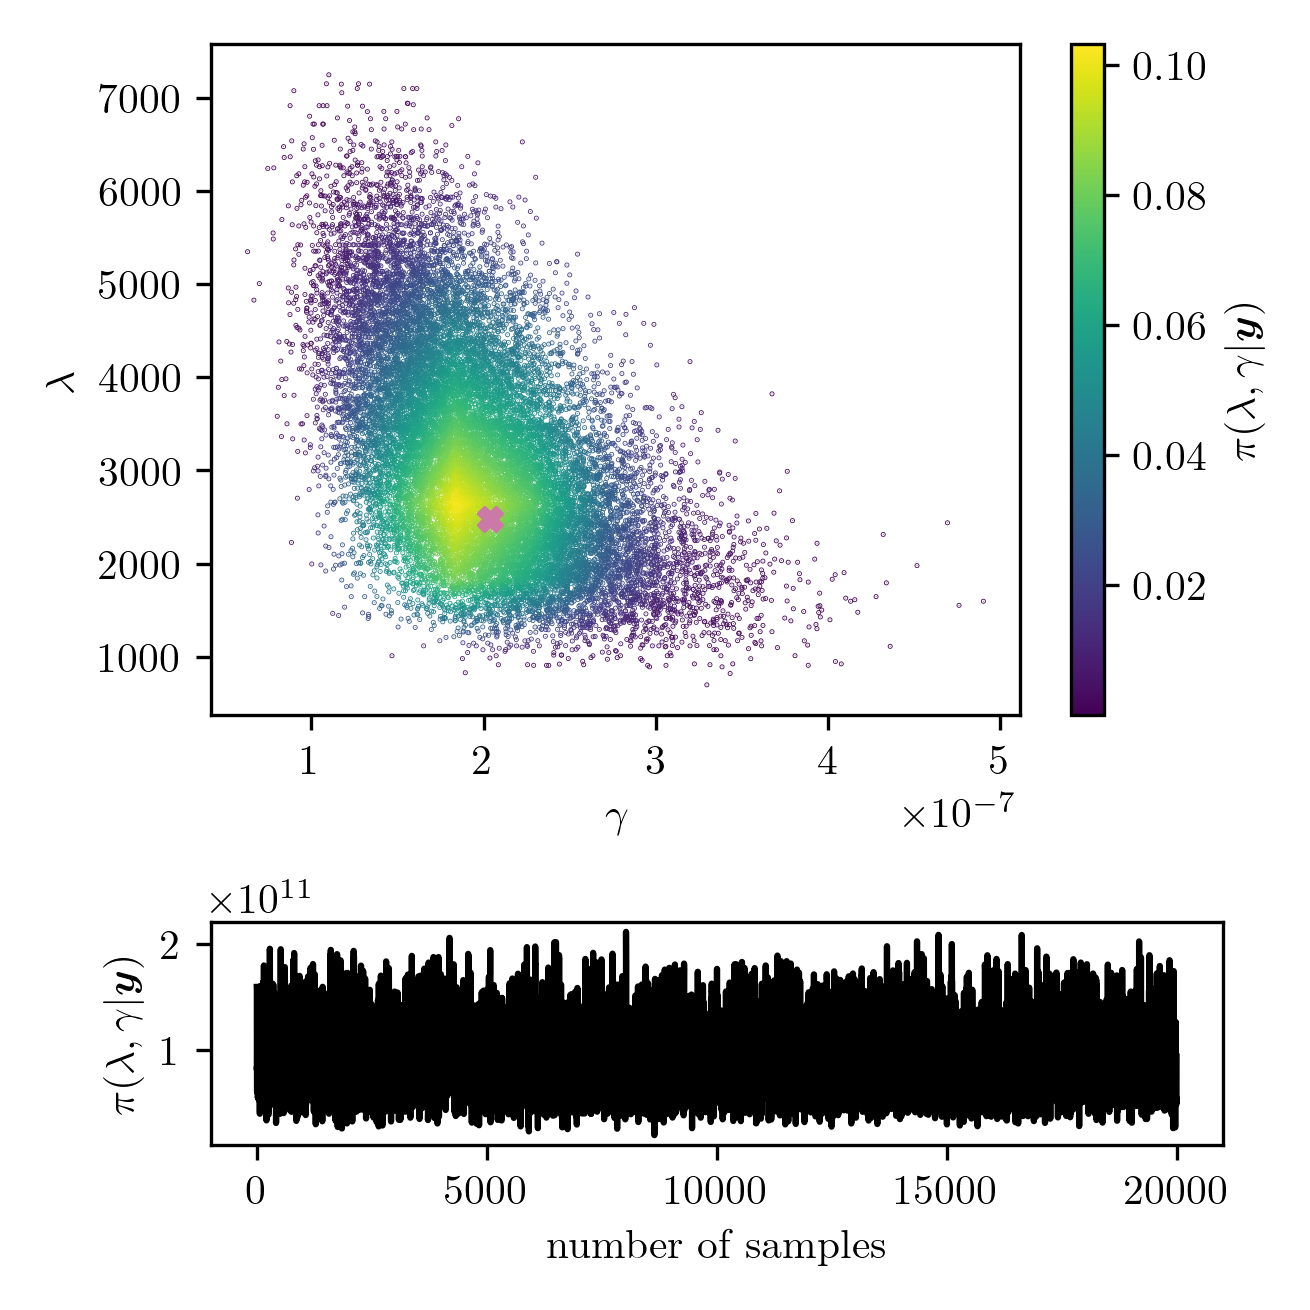
\includegraphics{ScatterplusHistoPlusTT.png}
	\caption[Samples from marginal posterior and TT approximation; trace plot of the MWG for $\pi(\lambda, \gamma| \bm{y})$]{Samples from the marginal posterior colour-coded using the TT approximation of $\pi(\lambda , \gamma  | \bm{y})$. The mode of $(\lambda_0 , \gamma_0)$ of $\pi(\lambda , \gamma  | \bm{y})$ is marked with the pink cross. To show ergodicity, we plot the trace of the samples of the MWG algorithm.}
	\label{fig:ScatterPlotTT}
\end{figure}
%\subsubsection{Sample from Marginal Posterior Distribution}
%\label{subsec:firstMarg}

%\begin{algorithm}[!ht]
%	\caption{Metropolis within Gibbs for $\pi(\lambda, \gamma | \bm{y})$}
%	\begin{algorithmic}[1]
	%		\STATE Initialise  \( \bm{\theta}^{(0)}  =( \lambda^{(0)} , \gamma^{(0)}  ) \) and set burn-in $N_{\text{burn-in}}$
	%		\FOR{ \( k = 1, \dots, N^{\prime} \)}
	%		\STATE Propose \( \lambda \sim \mathcal{N}(\lambda^{(t-1)}, 0.8 \lambda_0)  \)
	%		\STATE Compute
	%		\[ \alpha( \lambda  | \lambda^{(t-1)}) = \min \left\{ 1, \frac{\pi(\lambda | \gamma^{(t-1)}, \bm{y})  }{\pi(\lambda^{(t-1)}| \gamma^{(t-1)}, \bm{y})}  \right\} \]
	%		\STATE Draw $u \sim \mathcal{U}(0,1)$
	%		\IF{$\alpha \geq u$ }
	%		\STATE Accept and set \( \lambda^{(t)} = \lambda \)
	%		\ELSE  
	%		\STATE Reject and keep \(\lambda^{(t)} = \lambda^{(t-1)} \)
	%		\ENDIF
	%		\STATE Draw $\gamma^{(t)} | \lambda^{(t)} ,\bm{y} \sim \text{Gamma} \big( 0.5  \, m + 2, 0.5 \, f(\lambda^{(t)}) + 10^{-10}(1 + \lambda^{(t)}) \big) $
	%		\ENDFOR
	%		%\STATE Output: $ \bm{\theta}^{(N_{\text{burn-in}})}, \dots,  \bm{\theta}^{(k)} , \dots,   \bm{\theta}^{(N)} \sim \pi(\bm{\theta}| \bm{y}) $
	%		\STATE Output: $ (\lambda, \gamma)^{(N_{\text{burn-in}})}, \dots,  (\lambda, \gamma)^{(k)} , \dots,   (\lambda, \gamma)^{(N)} \sim \pi(\lambda, \gamma| \bm{y}) $
	%	\end{algorithmic}
%	\label{alg:margPost}
%\end{algorithm}



%
%We find the mode at the minimum of  $-\log\{ \pi(\lambda, \gamma | \bm{y}) \}$  using \texttt{scipy.optimize.fmin} function and limit the number of function evaluation to 25 and use Cholesky back and forward substitution to calculate values of $g(\lambda)$ and $f(\lambda)$.
%Additionally, we calculate $\bm{B}_0^{-1} \bm{L} $ and  $\bm{B}_0^{-1}  \bm{A}_L^T \bm{y}$ once more at $\lambda_0$ and plot the Taylor approximation within the sampling region in Fig. \ref{fig:fandg}.
%\subsection{Posterior distributions with Linear model for Ozone -- MTC}
%\label{sec:firstMTC}
%In this section we calculate the posterior marginal and then conditional (MTC) posterior distribution for ozone conditioned on the ground truth temperature and pressure profiles using the linear forward model $\bm{A}_L$.
%This is faster then the other way round (finding temperature over pressure conditioning on ozone) and temperature and pressure are well defined within the atmosphere so it is easier to just condition on a temperature and pressure profile out of a text book.
%We employ a so-called Metropolis within Gibbs (MWG) algorithm on the marginal posterior as summarised in the algorithmic Box \ref{alg:margPost} or use a Tensor-Train (TT) approximation to calculate marginal posterior values.
%Then we can either sample from the conditional posterior using the randomise then optimise (RTO) method or calculate conditional mean and variance using quadrature.
%The DAG in Fig. \ref{fig:DAGO3} visualises that process and we can show explicitly that we group the hyper-parameters $\delta, \gamma$ together to determine the marginal posterior $\pi(\gamma, \delta | \bm{y})$.
%Here $\gamma$ , the noise parameter, determines the noise precision $\bm{\Sigma} = \gamma ^{-1} \bm{I}$ and $\delta$, the smoothness parameter, the precision matrix $\bm{Q} = \delta \bm{L}$ of the prior distribution for $\bm{x}$.
%Then conditioned on the hyper-parameters the conditional posterior $\pi( \bm{x} |\gamma, \delta, \bm{y})$ gives the distribution of posterior ozone profiles.
%Note that we use the linear model $A_L$ here as we do not have an approximation to the non-linear model yet and all prior distributions are defined in Table \ref{tab:priors}.
%The full posterior $\pi(\bm{x},\gamma, \delta | \bm{y}) =  \pi(\bm{x}|\gamma, \delta ,\bm{y}) \pi(\gamma, \delta | \bm{y}) $ is given by multiplication of the marginal and conditional posterior densities. 
%\begin{align}
%	\bm{x} |  \bm{\theta}, \bm{y} \sim \mathcal{N} \Big(
%	\underbrace{\bm{\mu} + \left( \bm{A}^T \bm{\Sigma}^{-1} \bm{A} + \bm{Q} \right)^{-1} \bm{A}^T \bm{\Sigma}^{-1} (\bm{y} - \bm{A} \bm{\mu})}_{\bm{\mu}_{\bm{x} |  \bm{\theta}, \bm{y}}},
%	\underbrace{ \left( \bm{A}^T \bm{\Sigma}^{-1} \bm{A} + \bm{Q} \right)^{-1} }_{\bm{\Sigma}_{\bm{x} |  \bm{y}, \bm{\theta}}}
%	\Big) \, ,
%\end{align}
%is normal distribution and we compute weighted expectations, as in Eq.~\ref{eq:MargExpPos}, of the conditional mean and covariance matrix, where the weights are given by $\pi(\bm{\theta} | \bm{y})$. 
%Note that both the noise covariance $\bm{\Sigma} = \bm{\Sigma}(\bm{\theta})$ and the prior precision matrix $\bm{Q} = \bm{Q}(\bm{\theta})$ depend on the hyper-parameters $\bm{\theta}$.
\subsection{Full Conditional Posterior}
\label{subsec:firstCond}

Finally, we can evaluate the normally distributed full conditional posterior distribution
\begin{align}
	\bm{x}| \delta, \gamma, \bm{y}  \sim \mathcal{N}\big( \underbrace{ (\bm{A}^T \bm{A} + \delta / \gamma \bm{L} )^{-1} \bm{A}^T \bm{y}}_{\bm{x}_{\lambda}}, ( \underbrace{ \gamma \bm{A}^T \bm{A} + \delta \bm{L} }_{\gamma \bm{B}_{\lambda}}  )^{-1} \big) \, \label{eq:CondPost},
\end{align}
as in Eq. \ref{eq:CondPostLin}, with $\lambda = \delta / \gamma $.
\begin{figure}[ht!]
	\centering
	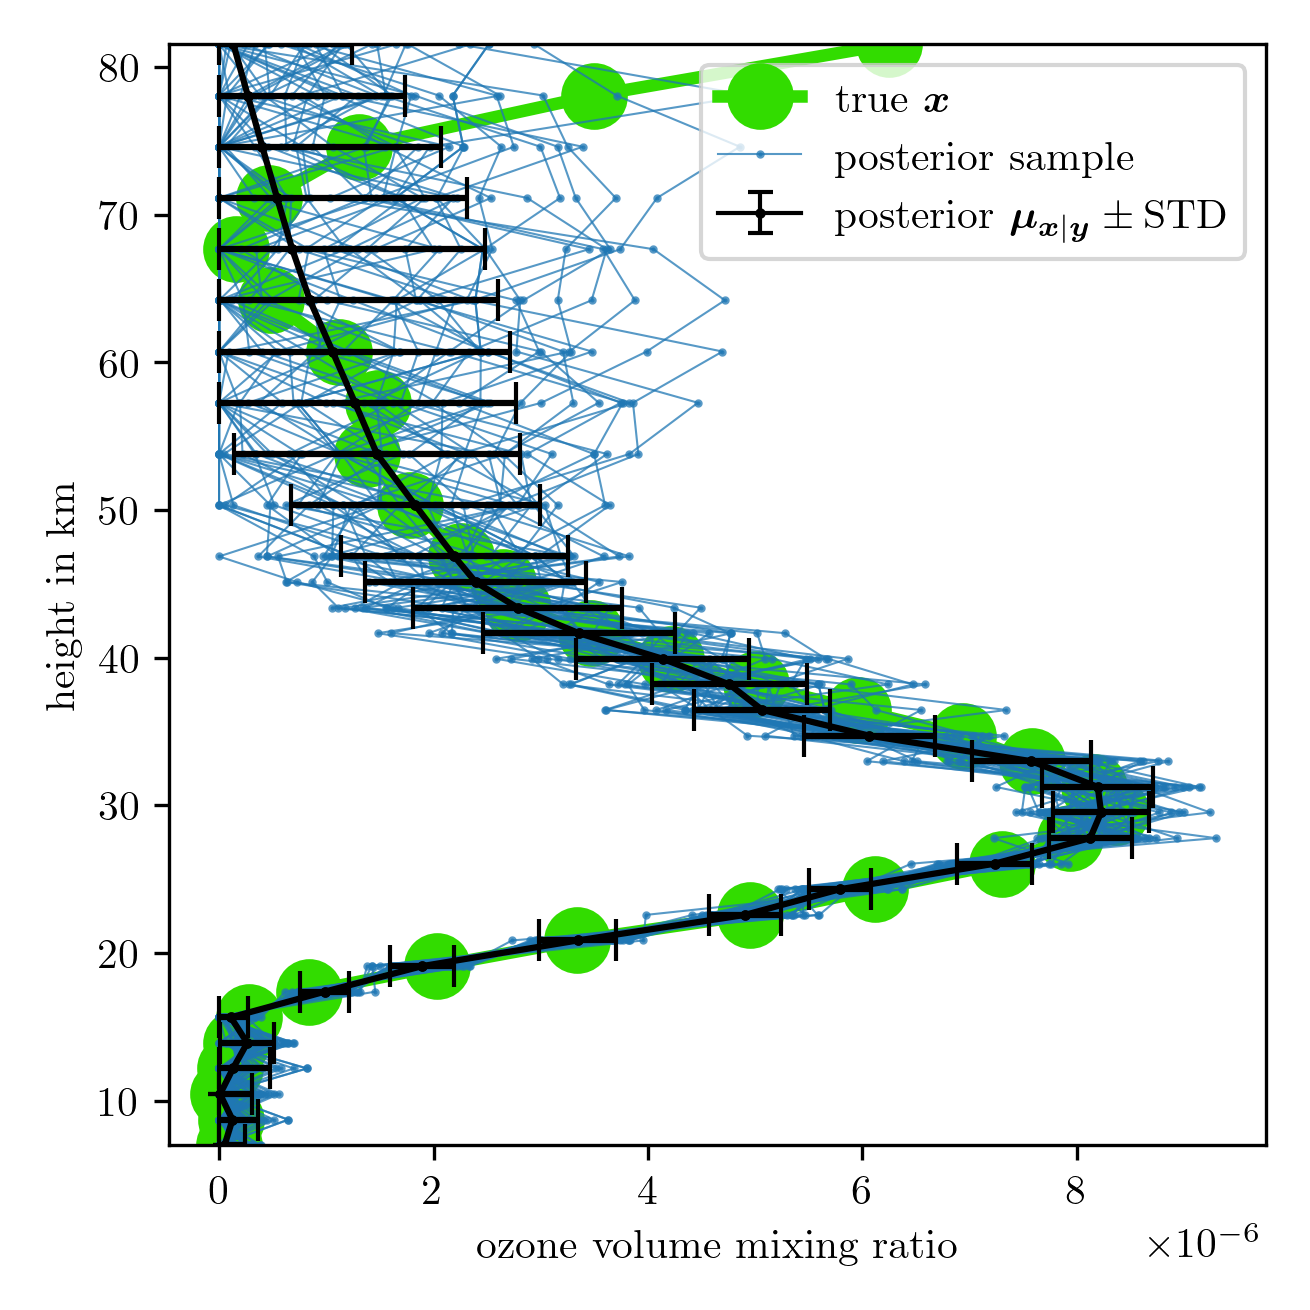
\includegraphics{FirstTestRes.png}
	\caption[Ozone samples of the full posterior.]{Ozone samples from the full posterior distribution $\pi(\bm{x}| \bm{y})$ after characterising posterior mean and covariance by weighted expectations over the marginal posterior $\pi(\lambda,\gamma | \bm{y})$ based on the linear forward map $\bm{A}_L$. We set negative ozone VMR values to zero.}
	\label{fig:O3Samp}
\end{figure}
In this thesis, we compute the posterior mean
\begin{align}
	\mu_{\bm{x}|\bm{y}} = \int \bm{x}_{\lambda} \pi(\lambda| \bm{y}) \diff\lambda \approx \sum \bm{x}_{\lambda_i} \pi(\lambda_i| \bm{y}) \, , \label{eq:MeanInt}
\end{align} and posterior covariance
\begin{align}
	\Sigma_{\bm{x}|\bm{y}} = \int \gamma^{-1}  \pi(\gamma | \bm{y} ) \, \diff \gamma \, \int  \bm{B}_{\lambda}^{-1} \, \pi(\lambda | \bm{y} )  \, \text{d} \lambda  \approx \sum {\gamma_i}^{-1}\pi(\gamma_i| \bm{y}) \sum \bm{B}_{\lambda_i}^{-1}\pi(\lambda_i| \bm{y})\, \label{eq:CovInt}
\end{align}
of $\pi(\bm{x}| \bm{y})$ as weighted expectations over the marginal posterior $\pi(\lambda,\gamma | \bm{y})$ by quadrature \cite[Sec. 2.1]{Dick_Kuo_Sloan_2013} with $\sum \pi(\lambda_i| \bm{y}) = \sum \pi(\gamma_i| \bm{y}) = 1$.
The weights $\pi(\lambda_i| \bm{y})$ and $\pi(\gamma_i| \bm{y})$ are either given by the TT approximation or by the bars of the sample-based histograms.
More precisely, the heights of the sample-based histogram bars act as quadrature weights, where $\lambda_i$ is defined at the centre of each bar.
We use Cholesky decomposition of $\bm{B}_{\lambda} = \bm{A}^T \bm{A} + \lambda \bm{L}$ to invert $\bm{B}_{\lambda}$ and to calculate $\bm{x}_{\lambda} = (\bm{A}^T \bm{A} + \lambda \bm{L} )^{-1} \bm{A}^T \bm{y}$ both via \texttt{scipy.linalg.cho\_solve}.
It is sufficient to evaluate $\bm{x}_{\lambda}$ and invert $\bm{B}_{\lambda}$ 20 times to obtain mean and covariance values of $\pi(\bm{x}|\bm{y})$ within a reasonable error (see Fig.~\ref{fig:MeanVarError}).
Finding the mode of $\pi(\lambda,\gamma|\bm{y})$, running the TT \texttt{cross}, calculating the marginals and the posterior mean and variance takes $0.025$s.
The MWG sampler takes $\approx0.5$s for the same results, so most computational effort lays within the sampling procedure and the time to calculate posterior mean and variance is negligible.
We plot posterior samples of $\pi(\bm{x}|\bm{y})$ in Fig.~\ref{fig:O3Samp} and set negative ozone values to zero, which is observed in almost every sample.
The fact that we have to deal with negative ozone values is due to the poor prior choice in $\pi(\bm{x}|\delta)$.
%Note that the sample mean is slightly larger than the posterior mean at heights where the data is noise-dominated, and the ozone values are determined by the prior, or where the ground truth is close to zero.
This indicates that one should use a different, more physically based prior or model a parametrised ozone profile.
Note that the posterior samples do not capture the second ozone peak at around $80$km.

If calculating the variance is too costly, the RTO method (see Sec.~\ref{subsec:RTO}) may be a feasible alternative to draw a sample from Eq.~\ref{eq:CondPost}.


%\subsubsection{Randomize then optimize -- RTO}
%For the RTO method we start by drawing an independent hyper-parameter sample $ ( \delta, \gamma) \sim \pi(\delta, \gamma | \bm{y})$ from the samples of the MwG.
%Then we generate two independent Gaussian random variables $\bm{v}_1 \sim \mathcal{N}(\bm{0},\gamma  \bm{A}^T_L \bm{A}_L)$ and $\bm{v}_2 \sim \mathcal{N}(\bm{0}, \delta \bm{L})$.
%Here  can use Cholesky factorisation of $\bm{L} =\bm{L}_C\bm{L}^T_C $ and the multiplication rule for normal distributions so that $\bm{v}_1 \sim \sqrt{\gamma} \bm{A}_L^T \mathcal{N}(0,\bm{I})$ and $\bm{v}_2 \sim \sqrt{\delta} \bm{L}_C \mathcal{N}(0,\bm{I})$.
%Then we solve
%\begin{align}
%	\label{eq:FirstRTO}
%	\left( \gamma \bm{A}_L^T  \bm{A}_L +\delta \bm{L} \right) \bm{x} = \gamma \bm{A}_L^T \bm{y} + \bm{v}_1 + \bm{v}_2 \, ,
%\end{align}
%using Cholesky back and forward substitution, for $\bm{x}$ and obtain one independent sample of $\pi(\bm{x}|\bm{y}, \bm{\theta})$.
%See Fig. \ref{fig:O3Samp}, where we plot $m = $ samples of the conditional posterior.
%
%The histogram in is binned as we intergate over it to 7 bins





\subsubsection{Eigenvalues full conditional posterior covariance}
\begin{figure}[ht!]
	\centering
	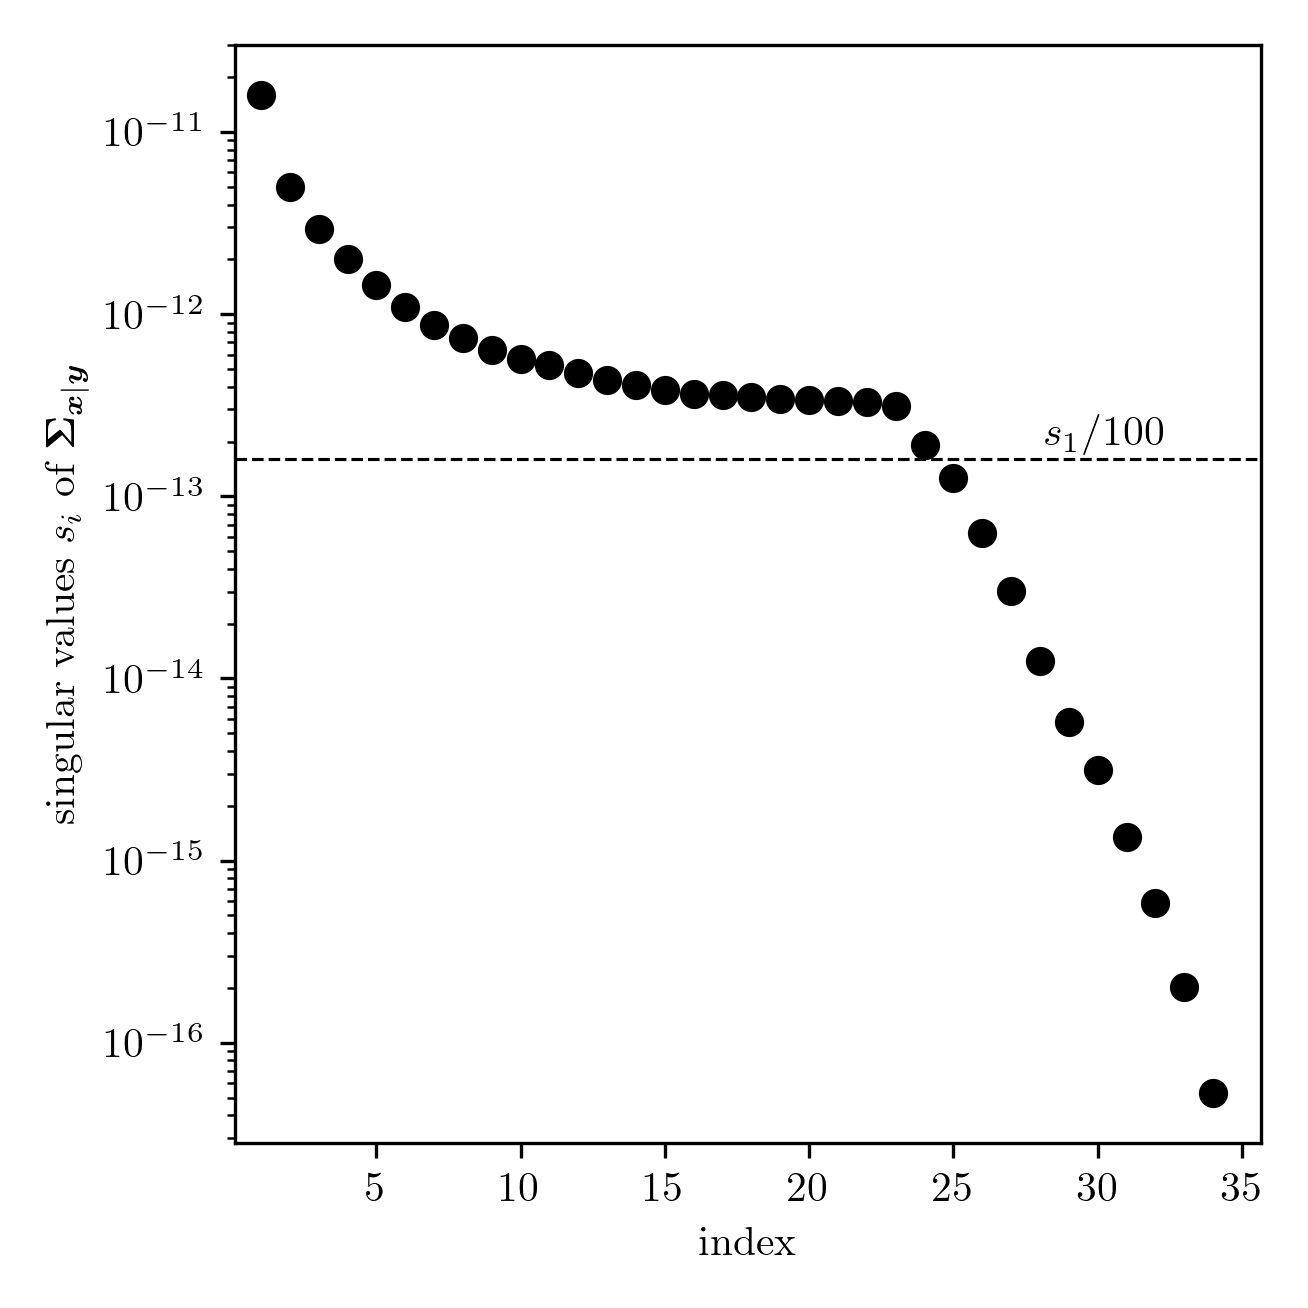
\includegraphics{CovSing.png}
	\caption[Eigenvalues of the posterior precision matrix]{Eigenvalues of the precision matrix of $\bm{Q}_{ \bm{x}|\delta, \gamma, \bm{y}}= \gamma \bm{A}^T \bm{A} + \delta \bm{L}$ of the full posterior distribution $\pi(\bm{x}|\delta, \gamma, \bm{y})$ for ozone.
		We see that large eigenvalues of $\gamma \bm{A}^T \bm{A}$ and $ \delta \bm{L}$ are rather unaffected by the prior compared to small eigenvalues.
		The eigenspace may differ.}
	\label{fig:PostCov}
\end{figure}
In Fig.~\ref{fig:PostCov} the eigenvalues (ordered in size) of the precision matrix $\bm{Q}_{ \bm{x}|\delta, \gamma,\bm{y}}=  \gamma \bm{A}^T \bm{A} + \delta \bm{L} $ for a random $\delta,\gamma \sim \pi(\delta,\gamma|\bm{y})$ are plotted and compared to the eigenvalues of the prior $\delta \bm{L}$ and the forward model $\gamma \bm{A}^T \bm{A}$.
We observe that the larger eigenvalues of $\bm{Q}_{ \bm{x}|\delta, \gamma,\bm{y}}$ are very much the same as the larger eigenvalues of $\gamma \bm{A}^T \bm{A}$.
Once the eigenvalues of $\gamma \bm{A}^T \bm{A}$ are significantly smaller than the eigenvalues of $\bm{Q}_{ \bm{x}|\delta, \gamma,\bm{y}}$ the structure of the eigenvalues is dominated by the eigenvalues of $\delta \bm{L}$.
The largest 10 eigenvalues of $\bm{Q}_{ \bm{x}|\delta, \gamma,\bm{y}}$ include ozone profile structure at lower altitudes, where the other eigenvector mainly represent structures at higher altitudes (see Fig.~\ref{fig:CovEigVec1} and Fig.~\ref{fig:CovEigVec1}).
Note that the eigenvalues of each matrix may correspond to different eigenvectors even if the eigenvalues of two matrices are the same.

\subsubsection{Errors of Full Posterior Mean and Covariance}
\begin{figure}[ht!]
	\centering
	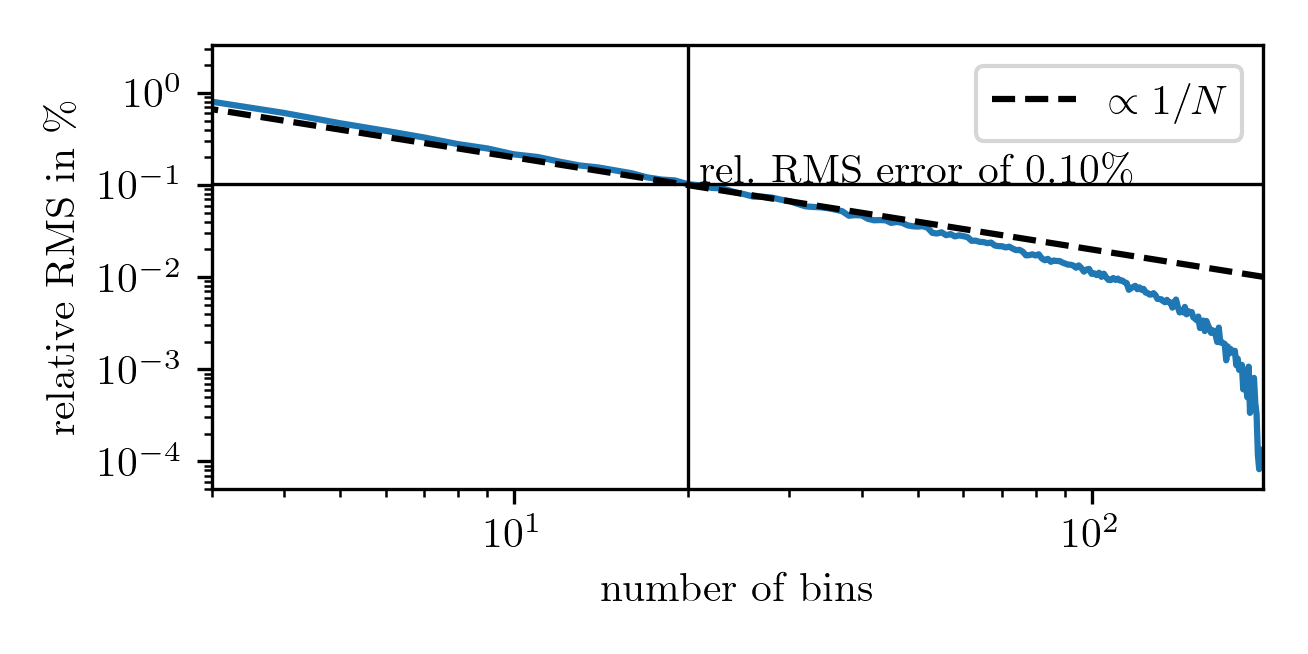
\includegraphics{relErrO3MeanVar.png}
	\caption[Relative Error of full posterior mean and covariance.]{Relative RMS error of $\bm{\mu}_{\bm{x}|\bm{y}}$ and covariance $\bm{\Sigma}_{\bm{x}|\bm{y}}$ calculated by the weighted expectations and compared to a ``ground truth'' given by weighted expectations over 200 bins.}
	\label{fig:MeanVarError}
\end{figure}
In Fig. \ref{fig:MeanVarError}, we plot the relative RMS error for the mean $\bm{\mu}_{\bm{x}|\bm{y}}$ and covariance $\bm{\Sigma}_{\bm{x}|\bm{y}}$ of $\pi(\bm{x}|\bm{y})$ due to grid size or number of bins of the marginal posterior.
Those results are obtained by calculating the weighted expectation over normalised histograms of $\pi(\lambda,\gamma | \bm{y})$, where the number of bins is increased and compared to a solution calculated from a histogram with 200 bins.
The relative error behaves roughly proportional to $1/N$, and we consider a relative RMS error less than $0.5\%$ good enough, which is easily met at 20 bins.
This sets the TT grid size and the number of evaluations of $\bm{x}_{\lambda}$ in Eq.~\ref{eq:MeanInt} and $(\gamma \bm{B}_{\lambda})^{-1}$ in Eq.~\ref{eq:CovInt}.
%marginal Ozone Pressure Temperature
%\clearpage


\section{Solution by Regularisation}
\label{sec:SolByReg}
Since we claim that the Bayesian approach is superior to regularisation methods, we compare the MTC method to a regularisation approach, which is most similar to our chosen linear-Gaussian Bayesian framework~\cite{fox2016fast}.

The regularised solution is defined as in~\cite{hansen2010discrete, fox2016fast} 
\begin{align}
	\bm{x}_{\lambda} =\underset{ \bm{x}}{\arg \min}\,  \lVert \bm{A}\bm{x} - \bm{y} \rVert_{L^2}^2 + \lambda \bm{x}^T \bm{L} \bm{x} \, ,
	\label{eq:XLam}
\end{align}
with the regularisation parameter $\lambda$, linear forward model matrix $\bm{A}$ and data $\bm{y}$.
A regularised solution
\begin{align}
	\bm{x}_{\lambda} = (\bm{A}^T\bm{A} + \lambda \bm{L} )^{-1} \bm{A}^T \bm{y} \label{eq:xLam} \, 
\end{align}
is calculated as in Sec.~\ref{sec:reg}.


To find the regularised solution, we use the L-curve method, and follow~\cite{hansen1993use}.
Within this method we compute $\bm{x}_\lambda$, for 200 different $\lambda$ values in between $10^{-8}$ to $10^{0}$ and plot the regularisation norm $\sqrt{\bm{x}_\lambda^T\mathbf{L} \bm{x}_\lambda}$ against the data misfit norm $\lVert \bm{A}\bm{x}_\lambda - \bm{x} \rVert_{L^2}$ (see Figure \ref{fig:LCurve}). 
The regularised solution corresponds to the ``corner'' of the L-curve at the point of maximum curvature provided by the kneedle algorithm~\cite{satopaa2011kneedle} using the function \texttt{kneed.KneeLocator} in $\approx 0.015$s, which is slightly faster then the TT approach to obtain full posterior mean and covariance.
The corresponding regularisation parameter is $\lambda = 1.6 \times 10^{-4}$.
\begin{figure}[ht!]
	\centering
	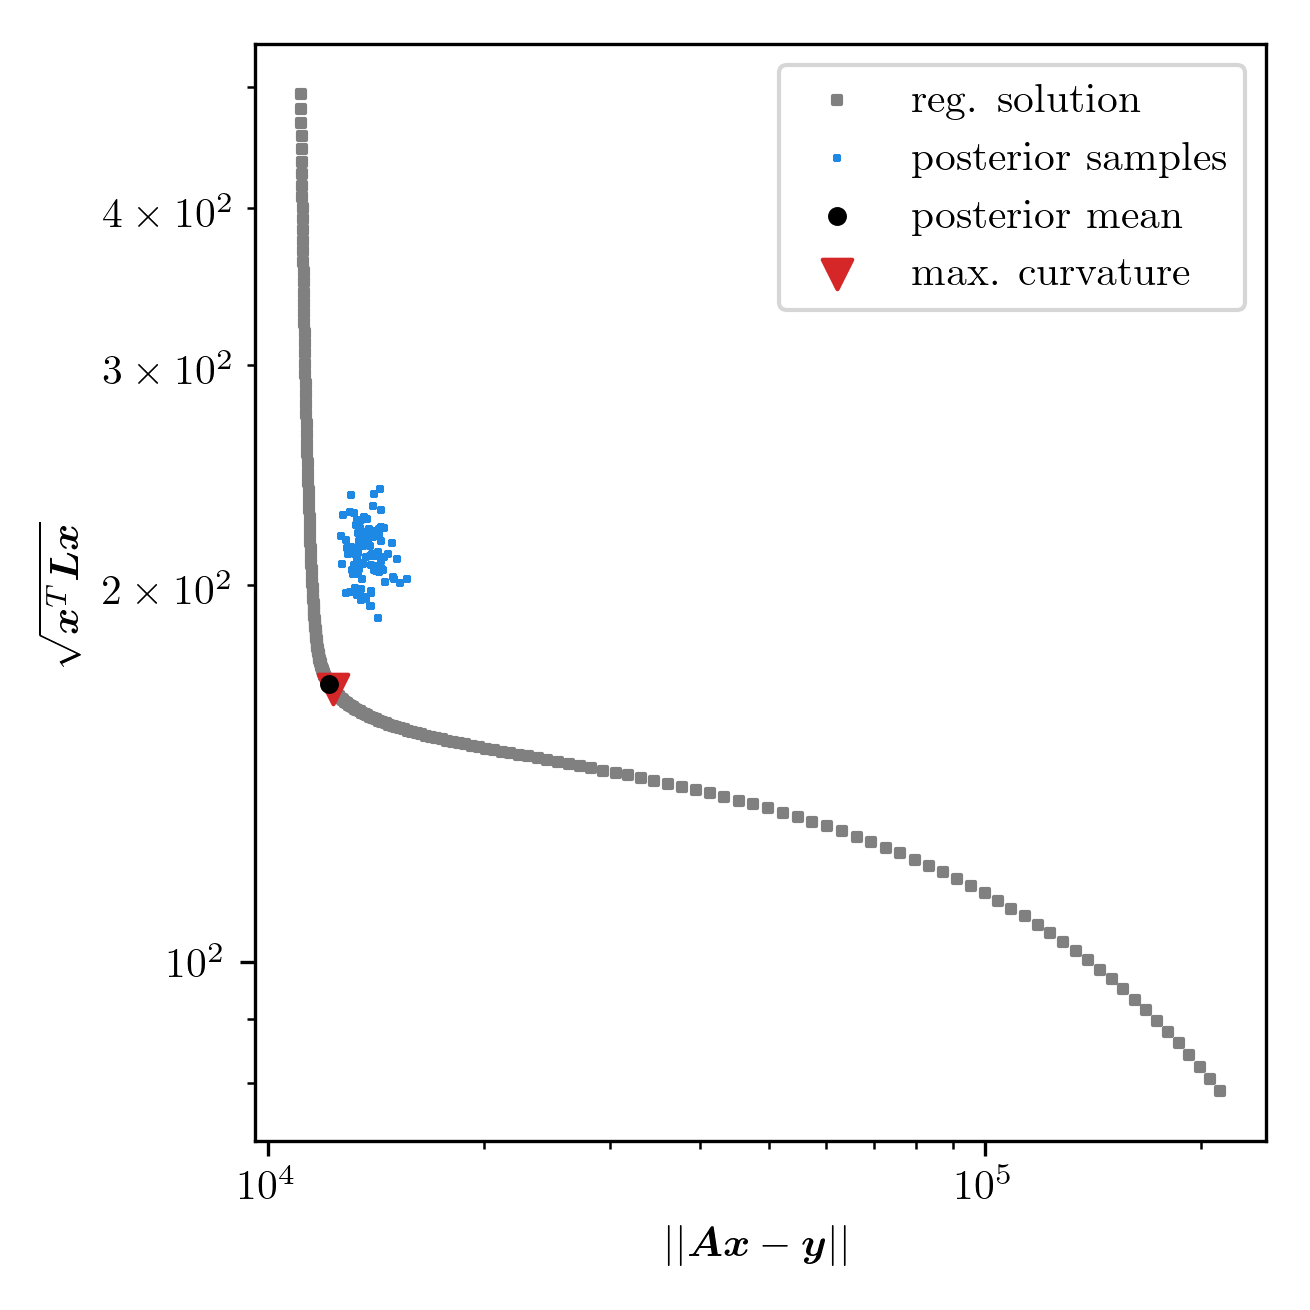
\includegraphics{LCurvePhD.png}
	\caption[Plot of the L-curve to find the regularised solution.]{L-Curve of regularised semi norm $\sqrt{\bm{x}^T\bm{Lx}}$ against the data misfit norm $\lVert \bm{A}\bm{x}_\lambda - \bm{x} \rVert_{L^2}$ for different $\lambda$ values, where $\bm{x}_{\lambda}$ is calculated as in Eq.~\ref{eq:xLam}. The best regularised solution is at the point of maximum curvature (pink triangle). Additionally, we calculate the data misfit norm and the regularised norm for the mean (black circle) and samples (blue squares) of the full posterior of ozone.}
	\label{fig:LCurve}
\end{figure}

The regularised solution in Fig.~\ref{fig:O3SolplsReg} is very similar to the posterior mean.
It is pretty clear that the regularised solution accounts for only one possible solution and does not provide uncertainties. The regularised solution is not similar to the samples drawn from the posterior $\pi(\bm{x}| \bm{y})$ (see Fig.~\ref{fig:O3Samp}).
The samples of $\pi(\bm{x}| \bm{y})$ plotted in Fig.~\ref{fig:LCurve} lie above the L-Curve, whereas the posterior mean and the regularised solution are on the L-Curve.
This does make sense, if one thinks about the mean as the (smooth) average over less-smooth samples and the regularised solution as an extremely smooth ozone profile (see Lagrangian in Sec. \ref{sec:reg}).
In contrast, the samples are less regularised and hence lie above the L-Curve, but have a similar data misfit norm, and as already mentioned, are all feasible solutions to the data.
Neither the regularisation solution nor the posterior ozone profiles capture the second ozone peak of the ground truth at high altitudes.
